\chapter{Experiments}
\label{ch:experiments}

\section{Datasets}
\label{sec:ds}

In this section we consider datasets that are separated in two opposing communities. The information about the opinions of each member of this community is known. Thus, we can assign internal opinions -1 and 1 to the nodes depending on their community membership\cite{tsapMatakosTerzi}.  We consider the following.

\begin{enumerate}

  \item The Karate dataset, that represents the friendships between the members of a karate club at a US university. This network is split in two equal size polarized communities around two rival karate instructors.
  
  \item The Books dataset, that is a network of US politics books. These books were published near the 2004 presidential election and sold by Amazon.com . These Books are classified as "Liberal", "Conservative", or "Neutral".  There are in total 43 liberal books, 49 conservative and 13 neutral.
  
  \item The Blogs dataset, a network of hyperlinks between online blogs on US politics. Blogs are classified as either Liberal or Conservative.
  
  \item The Elections dataset, this dataset is the network between the Twitter followers of Hillary Clinton and Donald Trump collected in the period 15/12/2016-15/01/2017 – around the time of the 2016 presidential elections. Members of this network are assigned an internal opinion of 1 or -1 based on which one of the two candidates they follow. We took a subsampled portion that has be done by Matakos, et al. !!cite here!!
  
  \item The beefban dataset, a  hashtag that Twitter users used in March 2015 to signal that their posts referred to a decision by the Indian government about the consumption of beef meat in India.
  
  \item The GermanWings dataset, a  hashtag that Twitter users used after the crash of Germanwings Flight 9525.
  
\end{enumerate}


\section{Experiments with heuristics}
\label{sec:experimHeuristics}

All experiments were made with an 2,7 GHz Dual-Core Intel Core i5 on the PyCharm IDE. We can only experiment with the $Karate$ and the $Books$ dataset on all the heuristics. The $Greedy$ algorithm cannot run on the rest of the datasets because they contain thousands of nodes. The $Greedy$ algorithm needs to consider changes in the network structure so it is impossible to compute the polarization so many times.
\\
\\ 
The same applies for the $GreedyBatch$ algorithm. Although the $GreedyBatch$ algorithm can run on the $beefban$ dataset that contains $799$ nodes it would take a lot of time even for the $polblogs$ dataset that has $1490$ nodes.
\\
\\
Only the $FirstTopGreedy$ and the $Expressed Opinion$ heuristics can run in all datasets but provide us with a small decrease in polarization. This decrease would be greater if we consider a bigger number of edge additions that are proportional to the size of the dataset. Greater number of edges would make $FirstTopGreedy$ nonrunnable. The $Expressed Opinion$ performs better in our datasets even in a big number of additions but still needs several hours. 
\\
\\
\clearpage

\subsection{Dataset statistics}

\begin{table}[H]
 \centering
 \caption{Stats}
 \label{tab:statistics}
 \begin{tabular}{| l || l | l | l | l |}
 \hline
  Name & \# of Nodes & \# of Edges & Avg. Degree & $\pi(z)$\\
  \hline
  \hline
  Karate & $34$ & $78$ & 4.5882 &  0.33964\\
  \hline
    books & $105$ & $441$ & 8.4 &  0.43429\\
  \hline
    beefban & $799$ & $6026$ & 15.0839 &  0.30326\\
  \hline
  polblogs & $1490$ & $16718$ & 22.4403 &  0.30983\\
  \hline
  GermanWings & $2111$ & $7329$ & 6.9436 &  0.44479\\
  \hline
  ClintonTrump & $2832$ & $18551$ & 13.1010 &  0.07582\\
  \hline
 \end{tabular}
 \end{table}
 
\vspace{20pt}

\subsection{A visualisation of edge additions in  the Karate dataset}

\vspace{20pt}

\begin{figure}[!htbp]
	\centering
	\captionsetup{justification=centering,margin=2cm}
	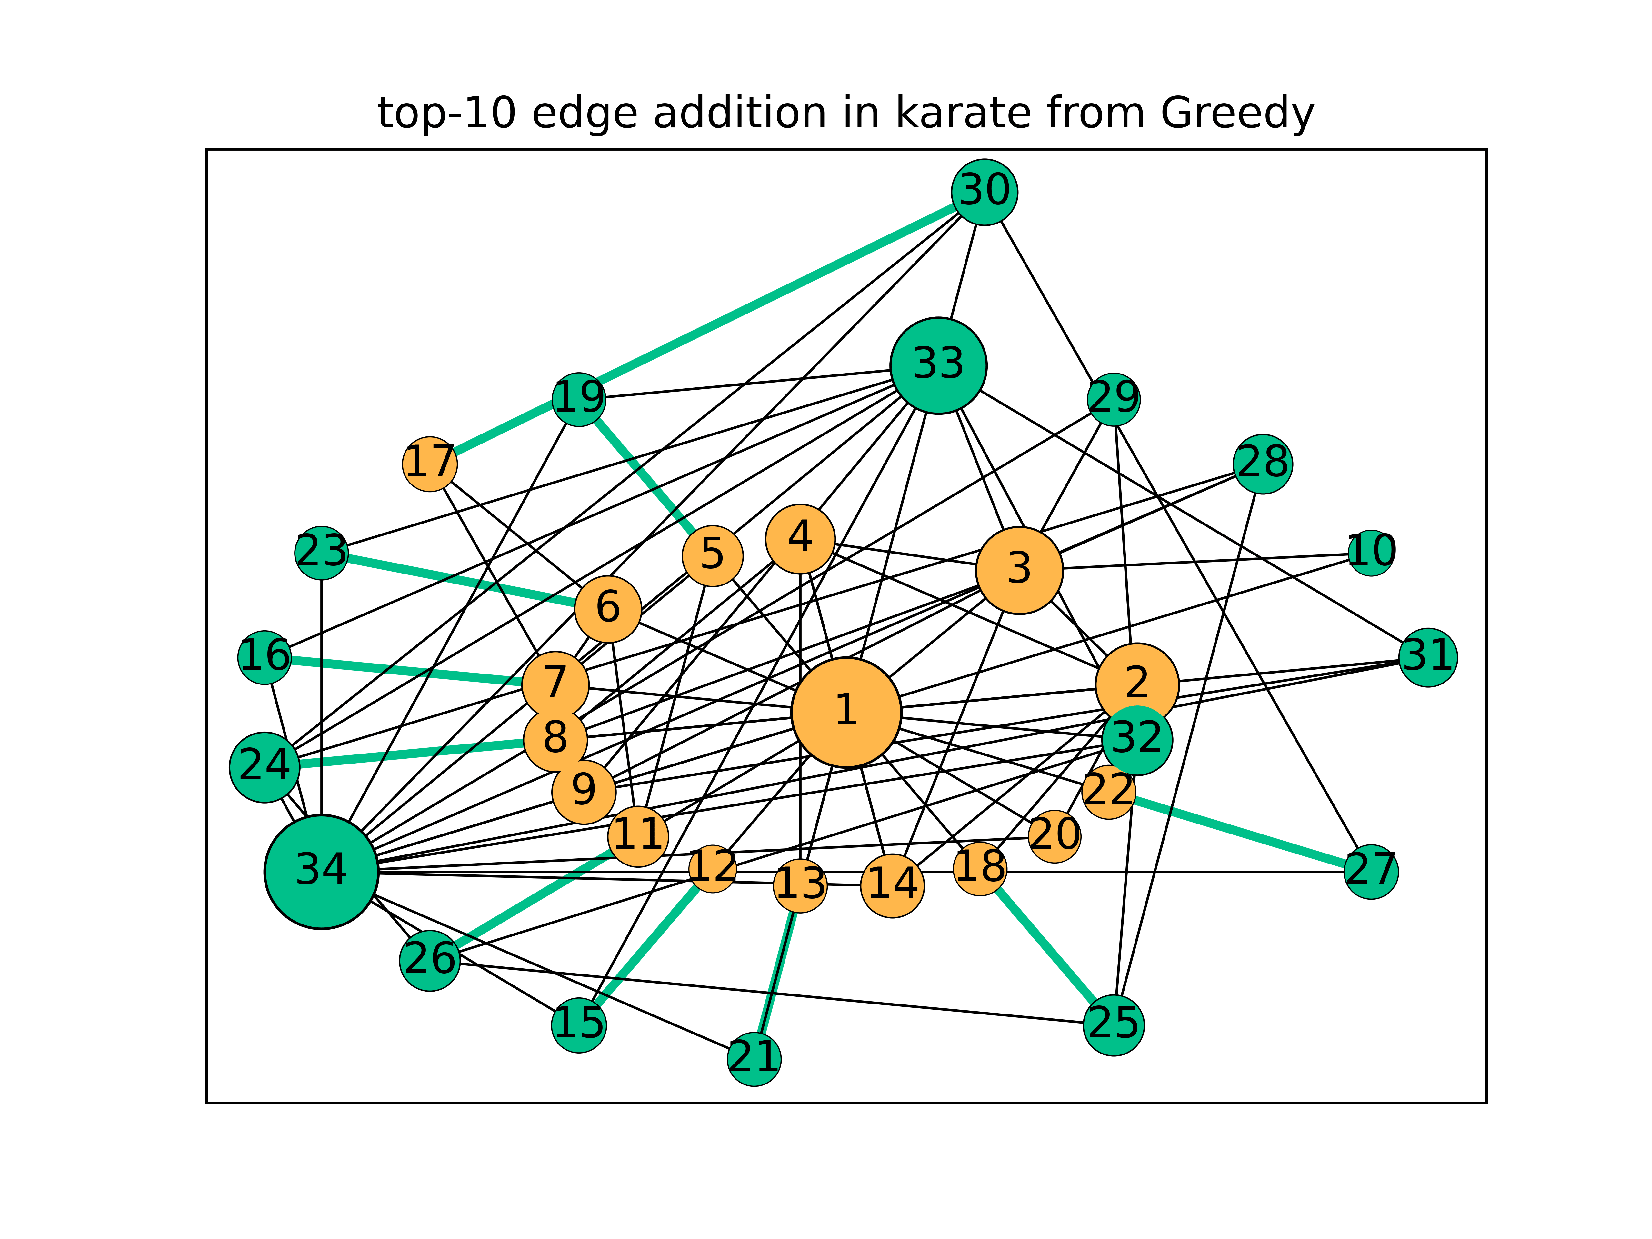
\includegraphics[width=0.65\textwidth]{Figures/top-10_karate_greedy}
	\vspace{20pt}
	\caption{the top-10 edges proposed by the greedy algorithm}
	\label{fig:top-10-karate}
\end{figure}

\clearpage


\subsection{Heuristics}


\begin{figure}[!htbp]
	\centering
	\captionsetup{justification=centering,margin=2cm}
	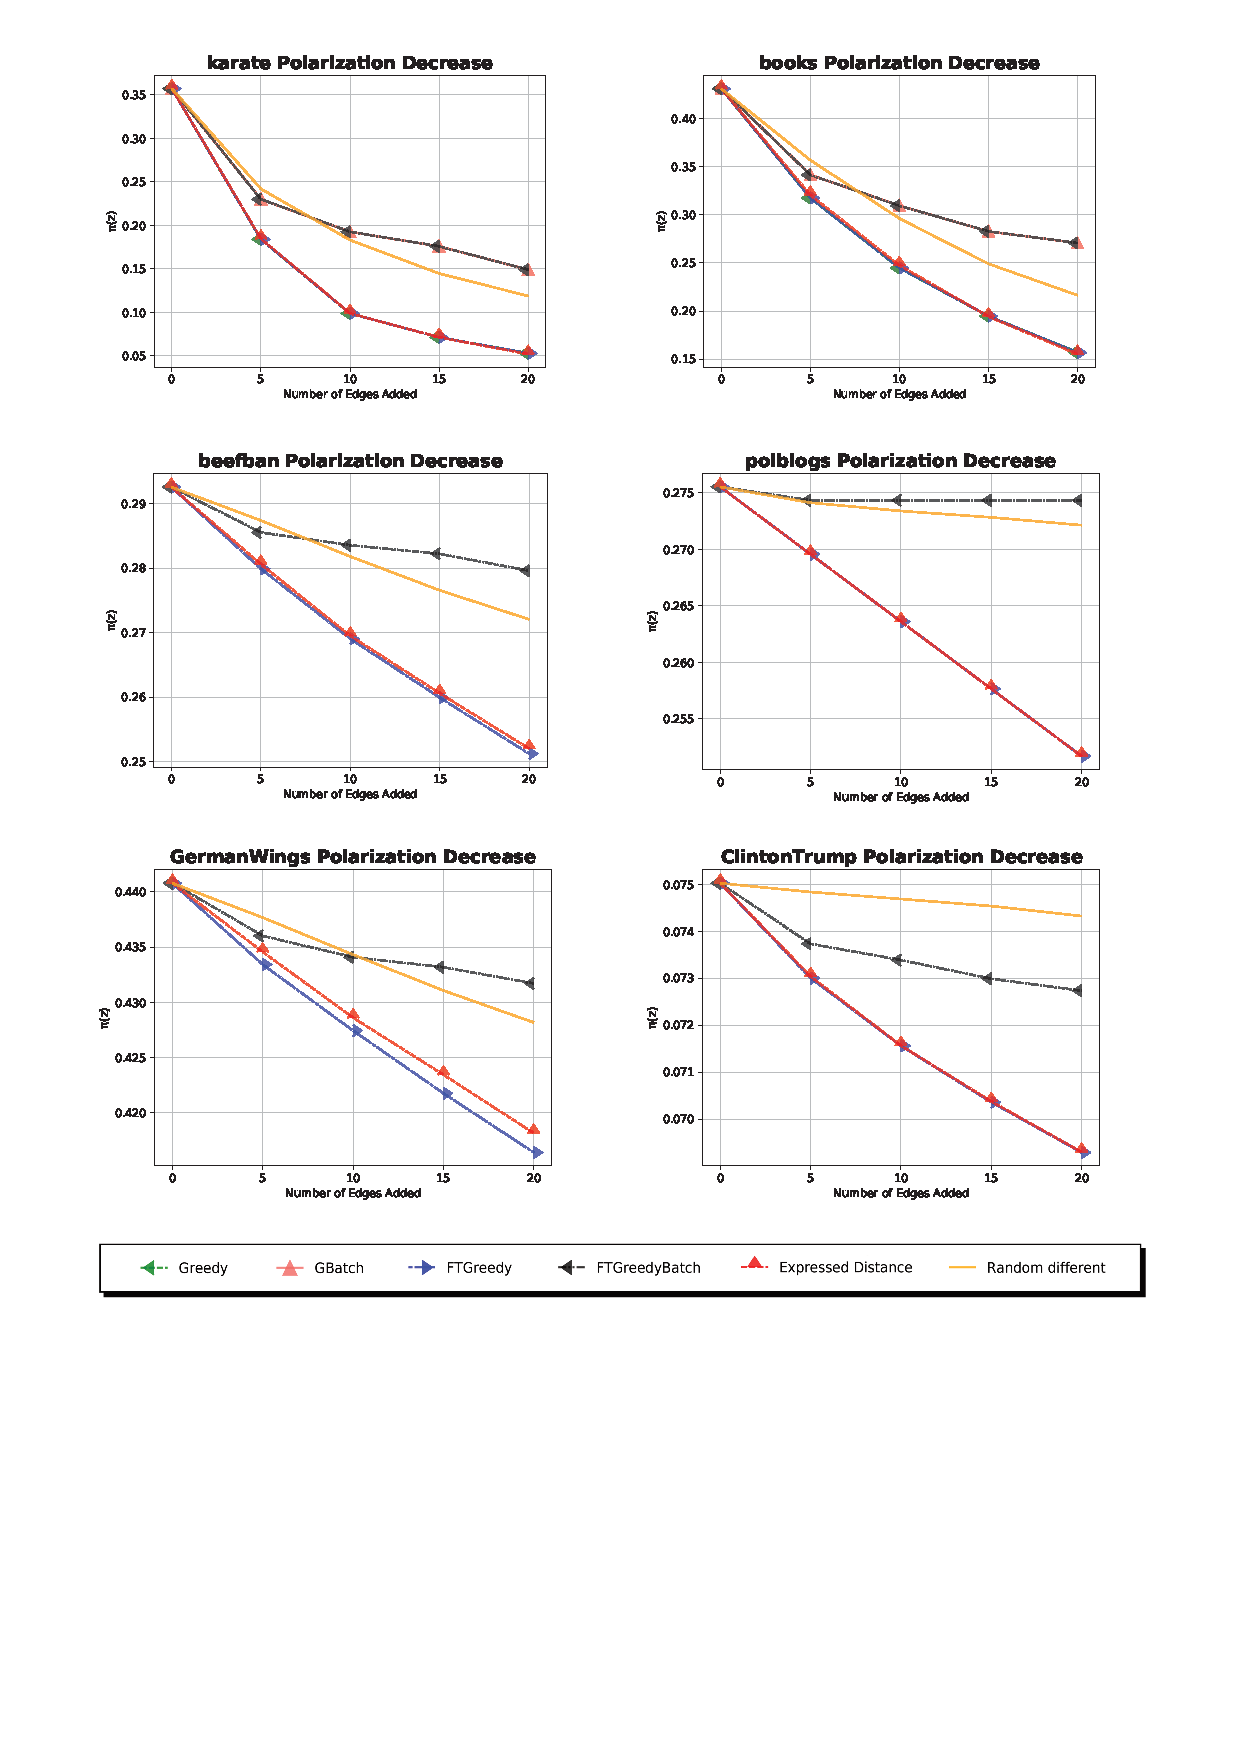
\includegraphics[width=0.90\textwidth]{Figures/heuristics_small}
	\caption{Comparison of the heuristics between datasets}
	\label{fig:heuristics_small}
\end{figure}




\section{Polarization decrease by removing edges}
\label{sec:polremovingdecrease}
Bellow we examine the removal of edges from a social graph and their result in polarization. We also find the edge betweenness centrality of each edge. 
\\
\\
The edge betweenness centrality is defined as the number of the shortest paths that go through an edge in a graph or network.(add cite Girvan and Newman 2002). 
\\
\\
In the tables following, Sign and Addition refer to the multiplication and the addition of the opinions of the nodes that are attached to the specific edge examined. Graphs in the books and blogs datasets, due to size, are omitted.
\\
\\

\subsection{Edges removal in the Karate dataset}

\begin{table}[H]
 \centering
 \caption{Edges with the biggest increase of polarization}
 \label{tab:edgesLargest}
 \begin{tabular}{| l || l | l | l | l |}
 \hline
  Edge & Betweenness Centrality & Polarization Increase & Sign & Addition\\
  \hline
  \hline
  (1, 32) & $0.12725$ & $0.04669$ & - &  0\\
  \hline
  (20, 34) & $0.059384$ & $0.03470$ & - &  0\\
  \hline
  (14, 34) & $0.06782$ & $0.02924$ & - &  0\\
  \hline
  (2, 31) & $0.03228$ & $0.02505$ & - &  0\\
  \hline
  (3, 28) & $0.04119$ & $0.02068$ & - &  0\\
  \hline
 \end{tabular}
  
 \caption{Edges with the biggest decrease of polarization }
 \label{tab:edgesLargest}
 \begin{tabular}{| l || l | l | l | l |}
 \hline
  Edge & Betweenness Centrality & Polarization Decrease & Sign & Addition\\
  \hline
  \hline
  (5, 11) & $0.00297$ & $5.55111*10^{-17}$ & + &  -2\\
  \hline
  (4, 8) & $0.00336$ & $3.04869*10^{-7}$ & + &  -2\\
  \hline
  (1, 4) & $0.02049$ & $1.38023*10^{-5}$ & + &  -2\\
  \hline
  (32, 34) & $0.05339$ & $1.61826*10^{-5}$ & + &  +2\\
  \hline
  (1, 8) & $0.02282$ & $1.93446*10^{-5}$ & + &  -2\\
  \hline
  \hline
 \end{tabular}
\end{table}

\begin{figure}[H]
	\centering
	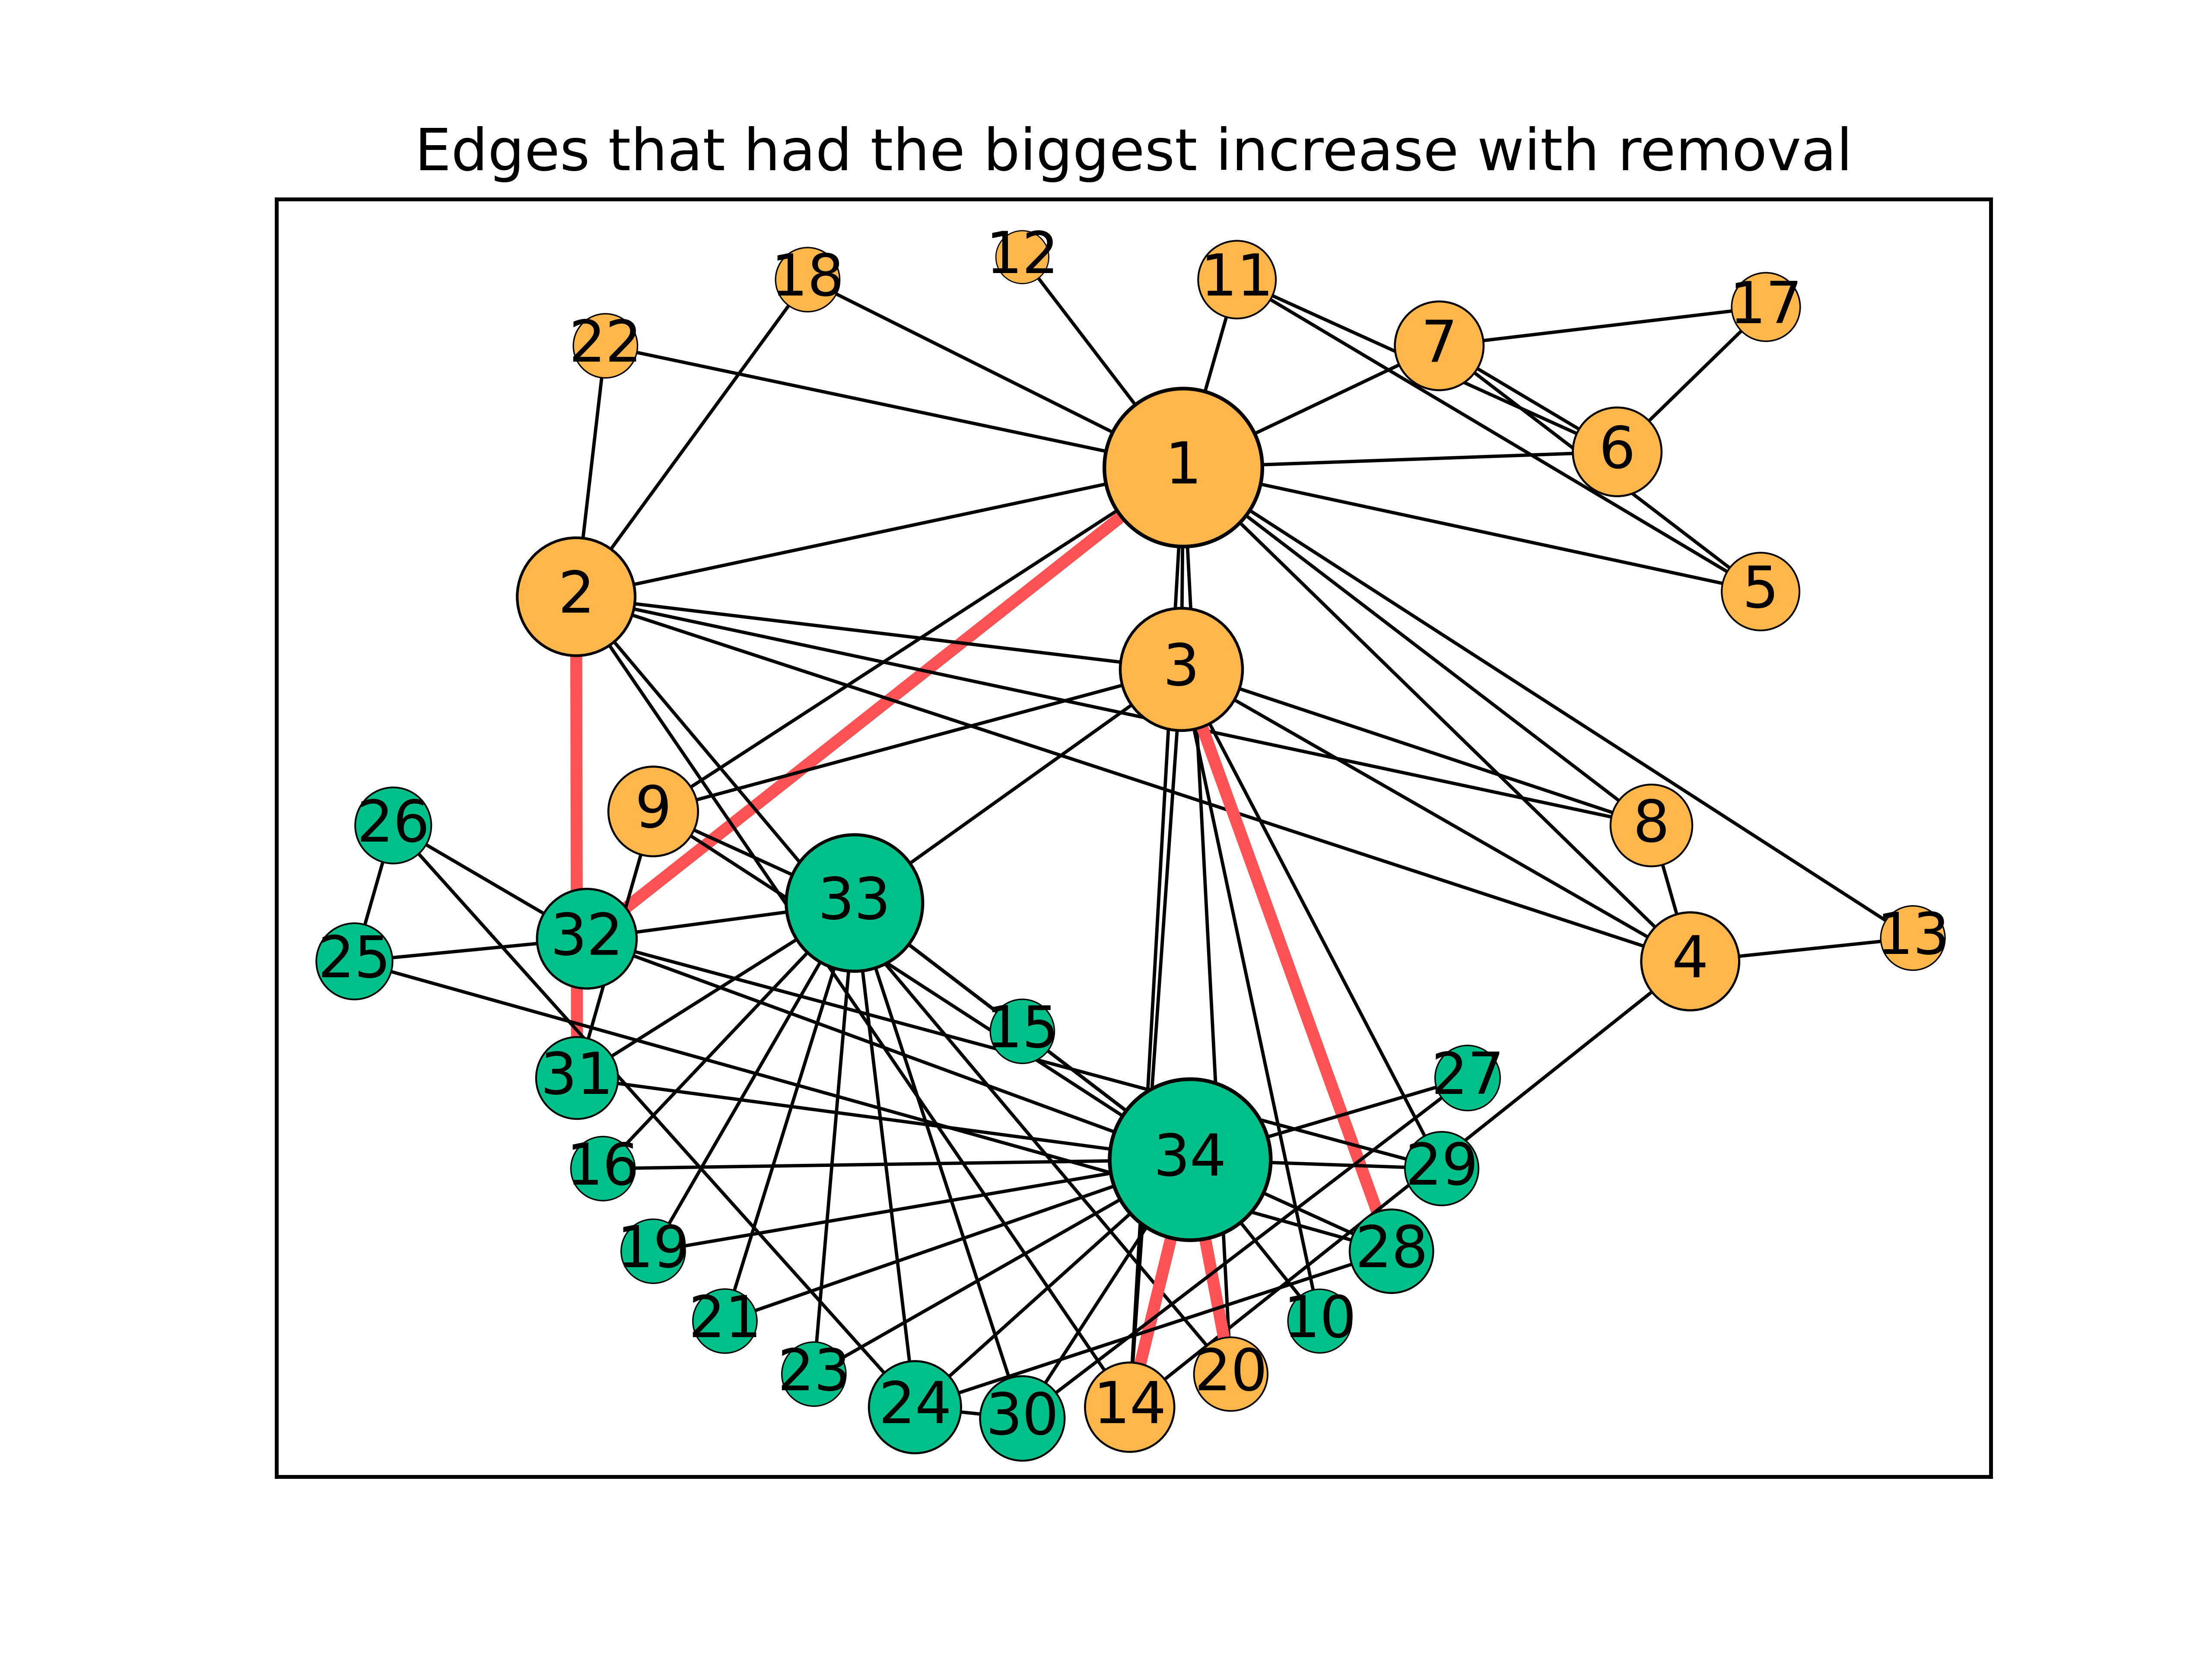
\includegraphics[width=0.65\textwidth]{Figures/karate_increase}
	\label{fig:karate_increase}
	\caption{Removing edges in Karate}
\end{figure}

\begin{figure}[H]
	\centering
	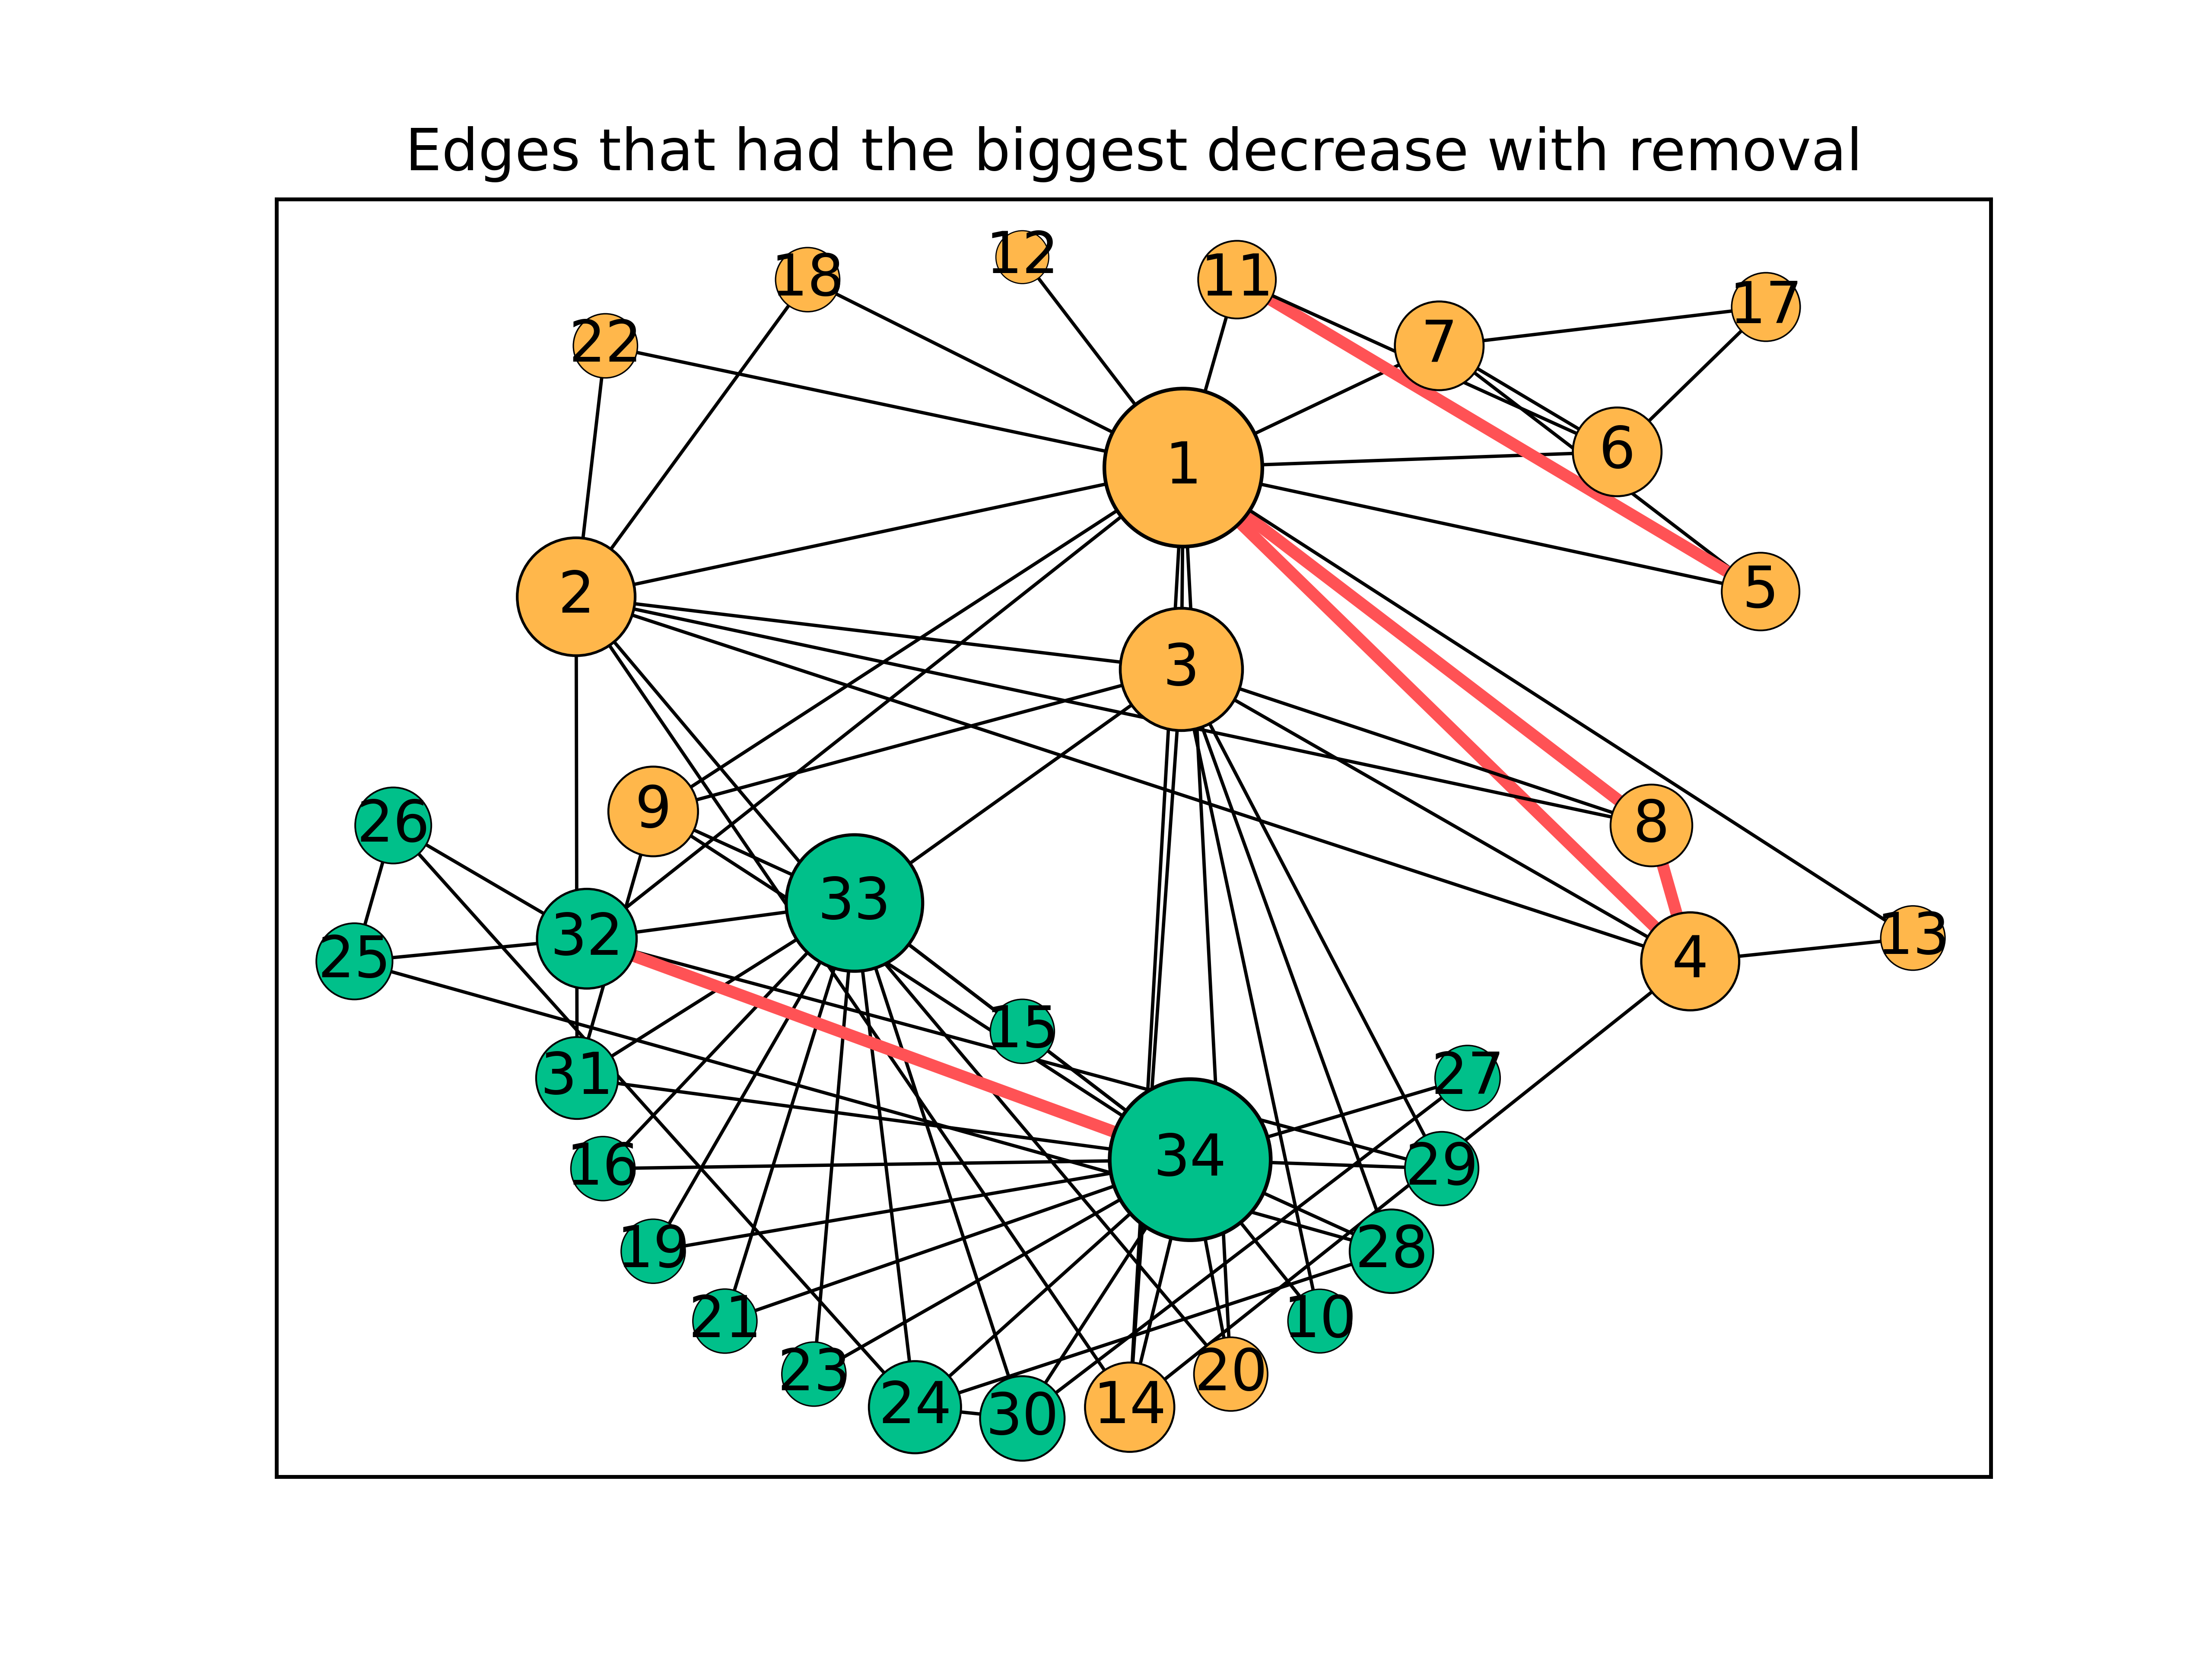
\includegraphics[width=0.65\textwidth]{Figures/karate_decrease}
	\label{fig:karate_decrease}
	\caption{Removing edges in Karate}
\end{figure}


\subsection{Edges removal in the Blogs dataset}

\begin{table}[H]
 \centering
 \caption{Edges with the biggest increase of polarization}
 \label{tab:edgesLargest}
 \begin{tabular}{| l || l | l | l | l |}
 \hline
  Edge & Betweenness Centrality & Polarization Increase & Sign & Addition\\
  \hline
  \hline
  (213, 793) & $0.00219$ & $0.00091$ & - &  0\\
  \hline
  (600, 1183) & $0.00439$ & $0.00074$ & - &  0\\
  \hline
  (523, 1375) & $0.00110$ & $0.00070$ & - &  0\\
  \hline
  (325, 1159) & $0.00110$ & $0.00069$ & - &  0\\
  \hline
  (632, 1000) & $0.00110$ & $0.00069$ & - &  0\\
  \hline
 \end{tabular}
 
 
 \caption{Edges with the biggest decrease of polarization }
 \label{tab:edgesLargest}
 \begin{tabular}{| l || l | l | l | l |}
 \hline
  Edge & Betweenness Centrality & Polarization Decrease & Sign & Addition\\
  \hline
  \hline
  (574, 1380) & $0.00014$ & $2.09620*10^{-6}$ & - &  0\\
  \hline
  (23, 1380) & $0.00021$ & $2.18102*10^{-6}$ & - &  0\\
  \hline
  (600, 1021) & $0.00024$ & $2.41460*10^{-6}$ & - &  0\\
  \hline
  (634, 1380) & $0.00010$ & $2.60119*10^{-6}$ & - &  0\\
  \hline
  (219, 1380) & $0.00014$ & $2.91467*10^{-6}$ & - &  0\\
  \hline
  \hline
 \end{tabular}
 
\end{table}

\subsection{Edges removal in the Books dataset}
\begin{table}[H]
 \centering
 \caption{Edges with the biggest increase of polarization }
 \label{tab:edgesLargest}
 \begin{tabular}{| l || l | l | l | l |}
 \hline
  Edge & Betweenness Centrality & Polarization Increase & Sign & Addition\\
  \hline
  \hline
  (0, 5) & $0.00056$ & $2.65885*10^5$ & - &  0\\
  \hline
  (7, 58) & $0.00713$ & $0.00012$ & - &  0\\
  \hline
  (5, 6) & $0.00222$ & $0.00012$ & - &  0\\
  \hline
  (6, 18) & $0.00858$ & $0.00014$ & +& -2\\
  \hline
  (0, 2) & $0.00031$ & $0.00349$ & - &  0\\
  \hline
 \end{tabular}
\end{table}

\begin{table}[H]
 \centering
 \caption{Edges with the biggest decrease of polarization}
 \label{tab:edgesLargest}
 \begin{tabular}{| l || l | l | l | l |}
 \hline
  Edge & Betweenness Centrality & Polarization Decrease & Sign & Addition\\
  \hline
  \hline
  (53, 76) & $0.06290$ & $0.01985$ & - &  0\\
  \hline
  (46, 102) & $0.04914$ & $0.01541$ & + &  -2\\
  \hline
  (19, 77) & $0.04367$ & $0.01458$ & + &  +2\\
  \hline
  (9, 51) & $0.02812$ & $0.01000$ & - &  0\\
  \hline
  (49, 72) & $0.06809$ & $0.00952$ & - &  0\\
  \hline
 \end{tabular} 
\end{table}

\subsection{Remarks about the edge removals}

We can clearly see that there is an association between the edge betweenness centrality and the decrease in polarization. Edges that contribute to a bigger decrease have larger betweenness centrality. 
\\
\\
A second thing that we see in all three datasets is that the biggest increase is coming from the removal of edges that connect opposing opinions.
\\
\\
In addition, during the experiments on the karate dataset, the removal of edge $(6, 7)$ had no effect on the polarization index. This leads to the following lemma.

\begin{lemma}
The polarization index can stay the same after an edge removal.
\end{lemma}

